% Figure M9-Zheng-68k hero: FACET on the 68k PBMC donor-A matrix with
% paper-published FACS-correlated per-barcode cell-type labels.
% Generated by experiments/m9_zheng68k.py --hero.
\begin{figure}[t]
 \centering
 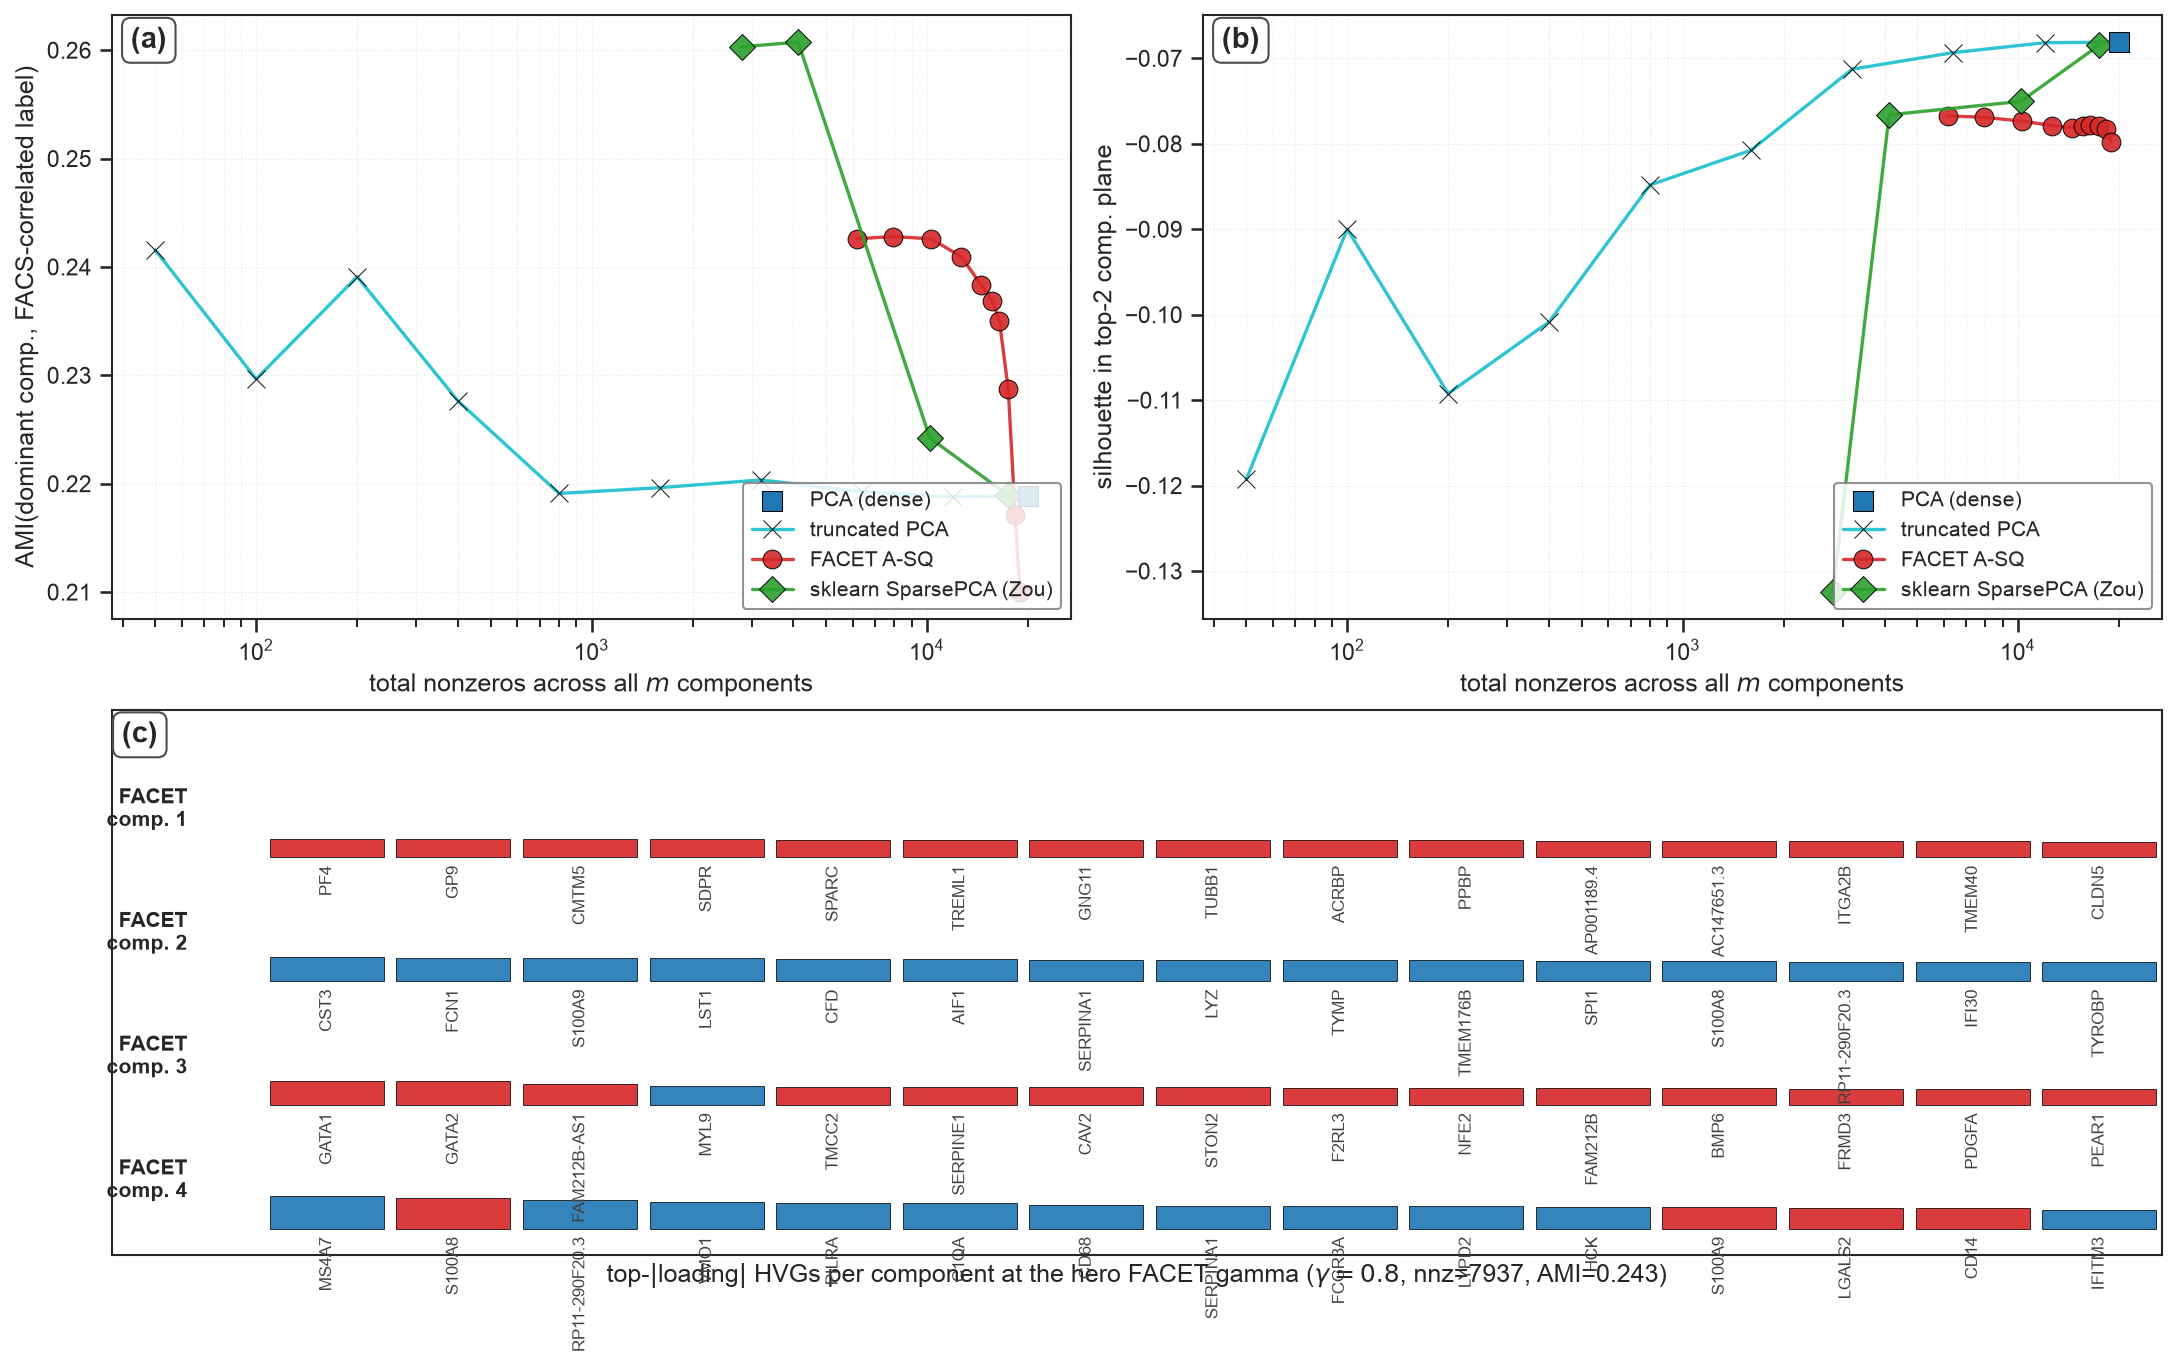
\includegraphics[width=\linewidth]{../shared/figures/generated/m9_zheng68k_hero.png}
 \caption{\textbf{M9 Zheng17 68k PBMC (donor A), native cell-type labels.} 68{,}551 cells $\times$ 2{,}000 HVGs; the per-barcode labels are the FACS-correlated cell-type assignments distributed with the Zheng et al.~2017 analysis repository, not derived from any clustering of this matrix. $m{=}10$ components. \textbf{(a)}~AMI vs total nonzeros: FACET A-SQ reaches AMI $0.243$ against the dense-PCA ceiling of $0.219$ ($+0.024$). \textbf{(b)}~Silhouette in the top-two component plane. \textbf{(c)}~Top-15 gene loadings per component at the hero FACET gamma; each component resolves into an immune programme consistent with its dominant cell type.}
 \label{fig:m9-zheng68k-hero}
\end{figure}
